The degradation of ECAL timing performance in the presence of out-of-time pileup motivates the development of a timing reconstruction method that explicitly accounts for overlapping pulses.
To address this, a cross-correlation (CC) timing algorithm has been developed that exploits the pulse amplitudes reconstructed by the multi-fit energy reconstruction.

The CC method uses the ten fitted pulse amplitudes, $A^{\mathrm{mf}}_{i}$, obtained from the multi-fit algorithm.
The measured pulse shape in a given crystal, denoted $H(\mathrm{BX})$, can be expressed as a linear superposition of contributions from the nominal in-time pulse and up to nine out-of-time (OOT) pulses originating from pileup interactions in neighboring bunch crossings.
Each of these contributions arises from scintillation light produced by particles incident in the crystal and is therefore expected to follow the same characteristic pulse shape.
While the amplitudes of these contributions are reconstructed by the multi-fit algorithm, the precise timing offset of each pulse relative to the nominal interaction is not known \emph{a priori}.

\begin{figure}[htbp]
\begin{center}
\resizebox{0.95\linewidth}{!}{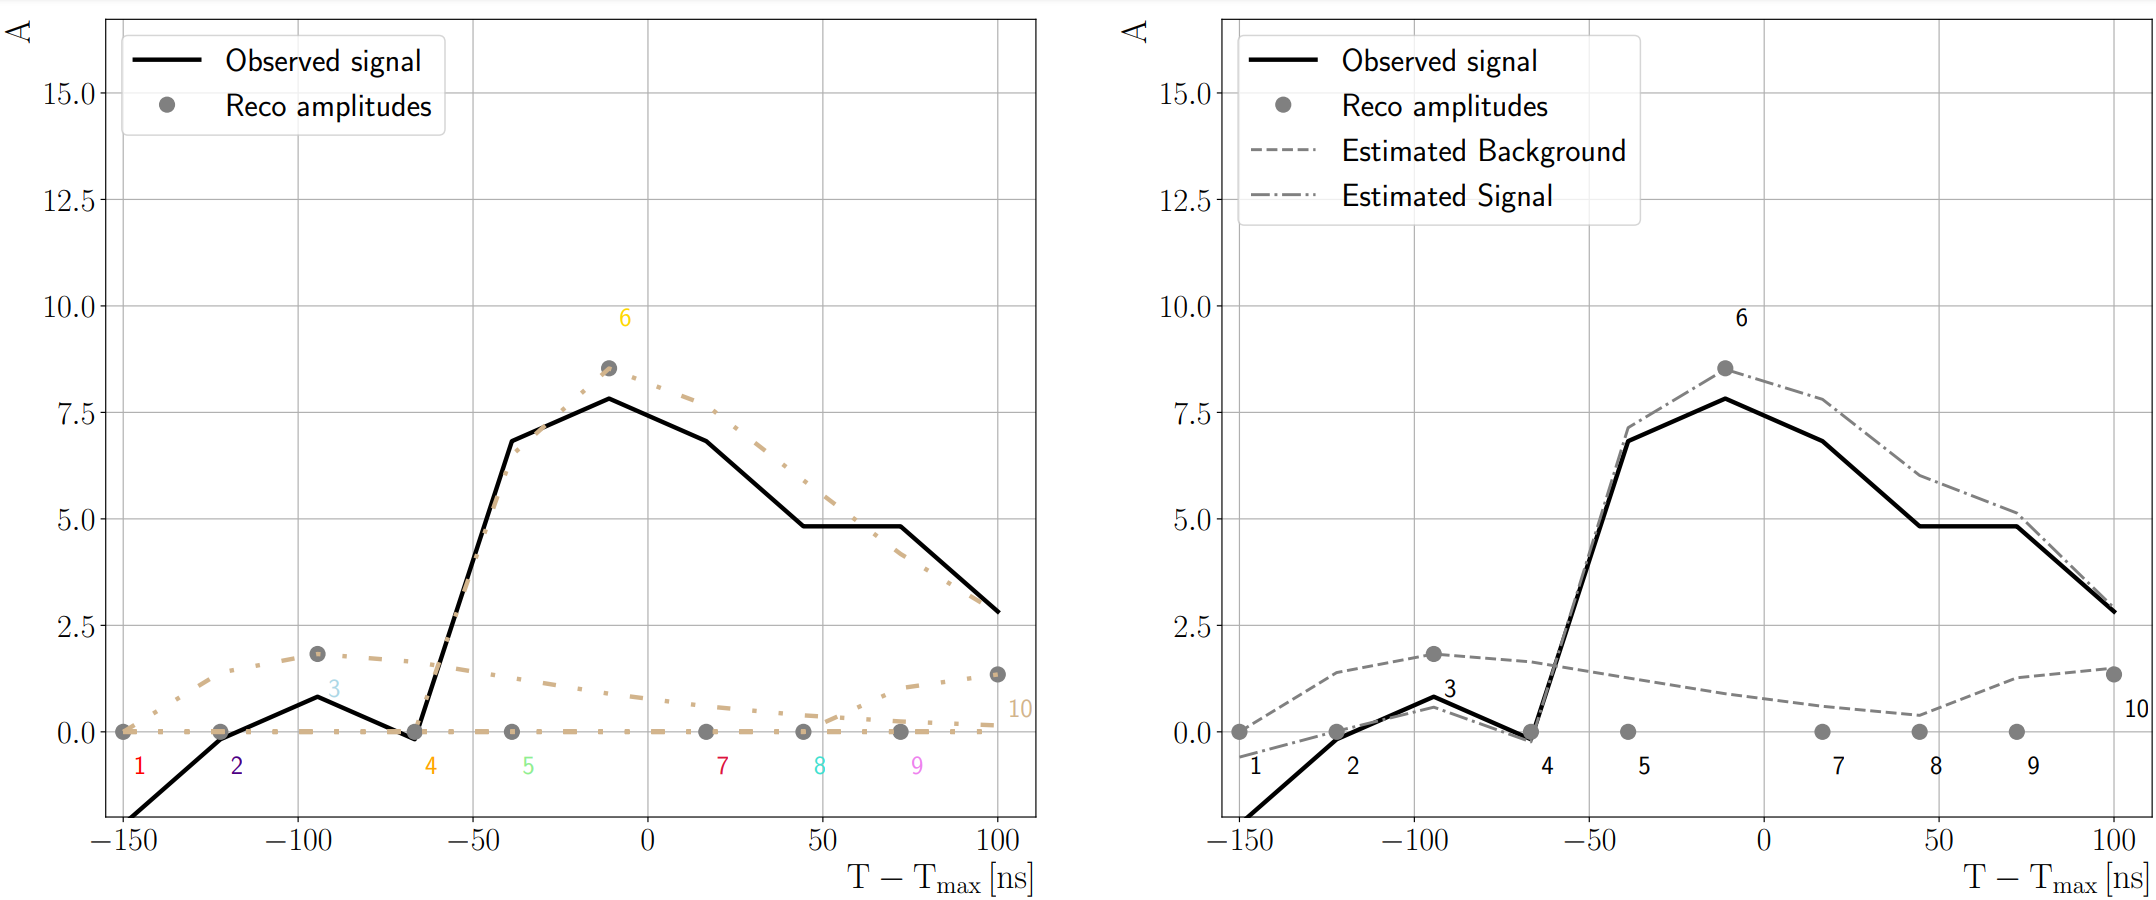
\includegraphics{fig/sec_algos/fOOT_reco_a2.png}}
\caption{Illustration of the OOT amplitude correction procedure used in the CC timing reconstruction.
In both panels, the solid black line shows the measured pulse shape $H(\mathrm{BX})$, and the black points indicate the fitted multi-fit amplitudes $A^{\mathrm{mf}}_{i}$.
Left: the reconstructed in-time and out-of-time pulse contributions $F^{\mathrm{OOT}}_{i}(A^{\mathrm{mf}}_{i},t)$.
Right: the background pulse shape $F_{\mathrm{bg}}(\mathrm{BX},t)$ obtained from the superposition of OOT contributions (dash-dotted line) and the recovered in-time signal $A^{\mathrm{sig}}(\mathrm{BX},t)$ after subtraction (dashed line).}
\label{tra_pulsereco}
\end{center}
\end{figure}

To enable continuous time shifts of the pulse shape, an analytic description of the characteristic ECAL pulse shape is constructed by fitting a parameterized function to the measured pulse templates on a channel-by-channel basis.
Using this analytic representation together with the fitted amplitudes $A^{\mathrm{mf}}_{i}$, a function
$F^{\mathrm{OOT}}_{i}(A^{\mathrm{mf}}_{i},t)$
is defined to describe the amplitude and time dependence of each OOT pulse contribution.
The total OOT background pulse shape is then obtained as the linear superposition
\begin{equation}
F_{\mathrm{bg}}(\mathrm{BX},t) =
\sum_{i} F^{\mathrm{OOT}}_{i}(A^{\mathrm{mf}}_{i},t) \, ,
\label{cc_bps}
\end{equation}
where the sum runs over all reconstructed OOT contributions.

The in-time signal pulse is recovered by subtracting the OOT background from the measured pulse shape,
\begin{equation}
A^{\mathrm{sig}}(\mathrm{BX},t) =
H(\mathrm{BX}) - F_{\mathrm{bg}}(\mathrm{BX},t) \, .
\label{cc_sig}
\end{equation}
If the correct timing parameters are used in the construction of $F^{\mathrm{OOT}}_{i}$, the recovered signal $A^{\mathrm{sig}}(\mathrm{BX},t)$ follows the expected characteristic pulse shape of an isolated scintillation signal.
This procedure is referred to as the \emph{OOT amplitude correction}.

The second step of the CC algorithm determines the arrival time of the in-time pulse by matching $A^{\mathrm{sig}}(\mathrm{BX},t)$ to the pulse shape template $S[\mathrm{BX}]$.
A normalized cross-correlation function is constructed,
\begin{equation}
d(\delta) \equiv
\frac{\sum_{\mathrm{BX}} A^{\mathrm{sig}}(\mathrm{BX},t)\,S(\mathrm{BX},\delta)}
     {\sqrt{\sum_{\mathrm{BX}} \left(A^{\mathrm{sig}}(\mathrm{BX},t)\right)^{2}}
      \sqrt{\sum_{\mathrm{BX}} \left(S(\mathrm{BX},\delta)\right)^{2}}} \, ,
\label{cc_delta}
\end{equation}
where $S(\mathrm{BX},\delta)$ denotes the pulse template shifted by a time offset $\delta$.
The reconstructed rechit time corresponds to the value of $\delta$ that maximizes the cross-correlation function $d(\delta)$.
This procedure is referred to as the \emph{cross-correlation fit}.

For reconstructed pulses with delays exceeding approximately 1\,ns, the OOT amplitude correction exhibits a systematic bias that leads to an underestimation of the reconstructed time.
This effect, and its impact on delayed signals, is discussed in detail in Section~\ref{sec:recobias}.
